% Input common header
\documentclass[xcolor=dvipsnames]{beamer}

\usecolortheme[named=Blue]{structure}
\setbeamertemplate{itemize items}[circle]

\usepackage{smartdiagram}


\author{Dr. Paul Larsen}
\date{\today}

\title{Risk, Artificial Intelligence and Discrete Geometry}
\begin{document}
\maketitle

\begin{frame}
\frametitle{Human are amazing at navigating a world that does not make sense}
\begin{tikzpicture}

  \node[inner sep=0pt] (grass) {
    \fbox{
        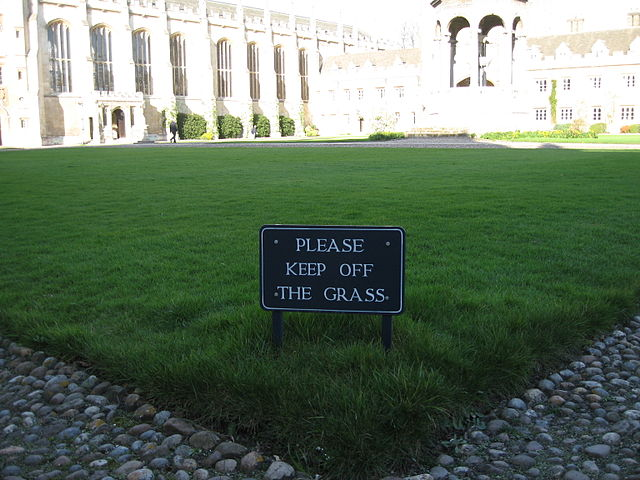
\includegraphics[width=0.7\textheight]{graphics/640px-Please_keep_off_the_grass_Great_Court_Trinity_College_Cambridge}
    }
  };
  \node[inner sep=0pt, right=0.5cm of grass] (door)  {
    
\includegraphics[width=.4\textheight]{graphics/keep_door_closed}
  };
   
\end{tikzpicture}

\end{frame}

%%%%%%%%%%%%
% AI Does Not Exist
%%%%%%%%%%%%
\begin{frame}[c]
  \begin{center}
  \huge Artificial Intelligence Does Not Exist
  \end{center}
  \end{frame}

\begin{frame}
\frametitle{Artificial Intelligence Does Not Exist, But ...}
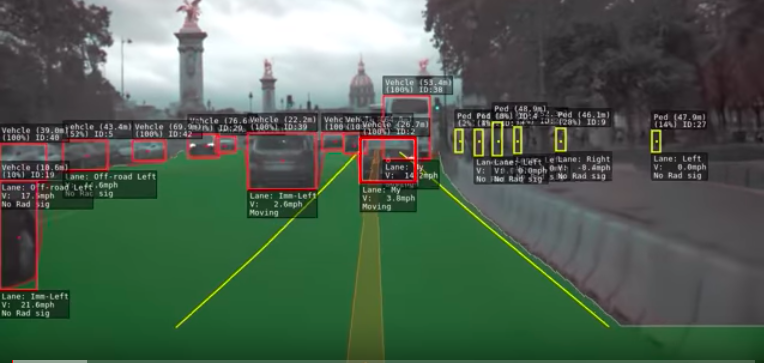
\includegraphics[width=\textwidth]{graphics/tesla_paris}

Source: \href{https://www.youtube.com/watch?v=_1MHGUC_BzQs}{YouTube: greentheonly, Paris streets in the eyes of Tesla Autopilot}
\end{frame}

\begin{frame}
\frametitle{Artificial Intelligence Does Not Exist, But ...}

\includegraphics[width=\textwidth]{graphics/google_duplex}

Source: \href{https://ai.googleblog.com/2018/05/duplex-ai-system-for-natural-conversation.html}{Google AI Blog}
\end{frame}

\begin{frame}
\frametitle{Artificial Intelligence Does Not Exist, But ...}
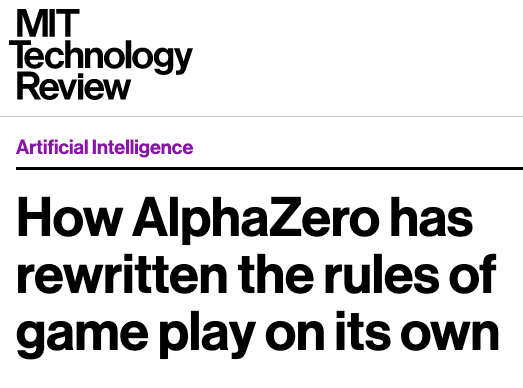
\includegraphics[width=0.8\textwidth]{graphics/alpha_go}

Source: \href{https://www.technologyreview.com/s/612923/how-alphazero-has-rewritten-the-rules-of-gameplay-on-its-own/}{MIT Technology Review}
\end{frame}

\begin{frame}
\frametitle{AI Struggles With Context}
The scientist named the population, after their distinctive horn, Ovid’s Unicorn. These four-horned, silver-white unicorns were previously unknown to science.\newline

Source: \href{https://www.lesswrong.com/posts/4AHXDwcGab5PhKhHT/humans-who-are-not-concentrating-are-not-general}{https://www.lesswrong.com/posts/4AHXDwcGab5PhKhHT/humans-who-are-not-concentrating-are-not-general}
\end{frame}

\begin{frame}
\frametitle{AI Struggles With Bias}
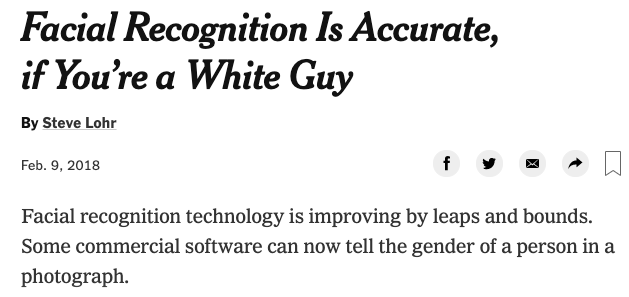
\includegraphics[width=\textwidth]{graphics/facial_bias}

Source: \href{https://www.nytimes.com/2018/02/09/technology/facial-recognition-race-artificial-intelligence.html}{New York Times}

See also: \href{https://www.theverge.com/2018/1/12/16882408/google-racist-gorillas-photo-recognition-algorithm-ai}{James Vincent, The Verge, Google 'fixed' its racist algorithm by removing gorillas from its image-labeling tech}
\end{frame}


\begin{frame}
\frametitle{AI Struggles With Human Behavior}
\href{run:graphics/siri_smart_sarcasm.m4a}{Siri Compliments}

\begin{center}
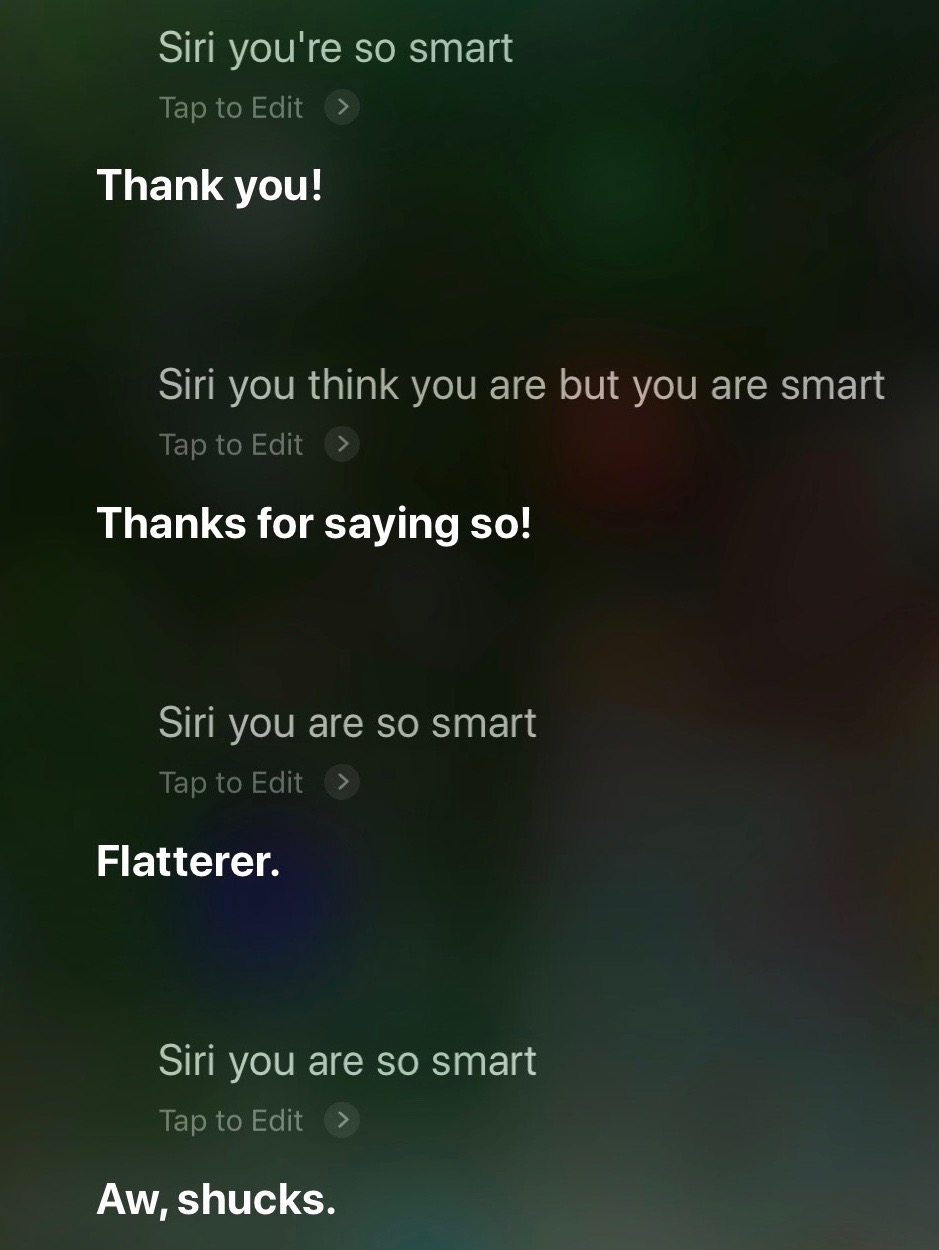
\includegraphics[height=0.7\textheight]{graphics/siri_transcript}
\end{center}
\end{frame}

\begin{frame}
\frametitle{Workshop topics}
\begin{enumerate}
\item Artificial intelligence for risk
\item Discrete geometry for artificial intelligence
\item Correlation and causation
\item Putting artificial intelligence into action
\end{enumerate}
\end{frame}

\begin{frame}
\frametitle{Workshop format}

\begin{itemize}
\item For each topic, lecture + tutorial
\item Emphasis on examples with data, thanks to python package \href{https://munichpavel.github.io/fake-data-for-learning/}{fake-data-for-learning}
\item Light on non-mathematical definitions, thanks to 
\end{itemize}
\centering

\includegraphics[width=0.3\textheight]{graphics/pi_wittgenstein}
\end{frame}

\begin{frame}
  \frametitle{Artificial intelligence in insurance}

  \begin{itemize}
    \item Underwriting: selling insurance, e.g. using a \emph{technical pricing model} that predicts expected claims
    \item Claims: dealing with client loss events, e.g. using algorithmic \emph{straight-through-processing} or \emph{fraud detection}
    \item Operations: process efficiency
  \end{itemize}
\end{frame}

\begin{frame}
\frametitle{Good Market Understanding Trumps Technology}
\centering
\smartdiagramset{
	back arrow disabled=true,
}
\smartdiagram[flow diagram:verticall]{Market,
  Data, AI}
\end{frame}

\begin{frame}
  \frametitle{Model selection: theory sketch}
  Goal: select the best model for data to come, i.e. minimize \emph{generalization error}.\newline

  Basic steps
  \begin{itemize}
    \item {\color{blue}Split data} set into train, validation and test sets
    \item For each model family (e.g. logistic regression, gradient boosted tree classifier), {\color{blue}select features} and {\color{blue}optimize model parameters} on training data
    \item For each model family, {\color{blue}evaluate fitted models} on validation set with chosen metric (e.g. recall, accuracy) and choose best
    \item To {\color{blue}estimate generalization error}, evaluate the best model on the test set.
  \end{itemize}
\end{frame}

\begin{frame}
\frametitle{Model selection example: hit rate for insurance quotes}
Fake data generated with \href{https://munichpavel.github.io/fake-data-for-learning/}{fake-data-for-learning}\newline

 \begin{tabular}{lrrr}
\toprule
product\_type &  days &  rating &  hit \\
\midrule
    property &     3 &       1 &    0 \\
   liability &     1 &       0 &    0 \\
   financial &     0 &       1 &    0 \\
   liability &     3 &       0 &    0 \\
   liability &     0 &       0 &    1 \\
\bottomrule
\end{tabular}
\newline

 Variables
\begin{itemize}
\item product\_type: Client line of business
\item days: Number of days to generate quote
\item rating: Binary indication of client risk
\item hit: Binary, 1 for success (binding the quote), 0 for failure
\end{itemize}
\end{frame}


\begin{frame}
\frametitle{Model selection example: lightning data}
Fake data generated with \href{https://munichpavel.github.io/fake-data-for-learning/}{fake-data-for-learning}\newline

 \begin{tabular}{lrr}
\toprule
     city &  year &  lightning\_strike \\
\midrule
 Ljutomer &  1990 &                 0 \\
 Turnišče &  1990 &                 0 \\
  Velenje &  1990 &                 0 \\
  Vrhnika &  1990 &                 0 \\
 Jesenice &  1990 &                 0 \\
\bottomrule
\end{tabular}
\newline

 Variables
\begin{itemize}
\item city: Slovenian city
\item year: calendar year AD
\item lightning\_strike: Number of lightning strike deaths per year
\end{itemize}
\end{frame}

\begin{frame}
\frametitle{Model selection example: university admissions data}
Fake data generated with \href{https://munichpavel.github.io/fake-data-for-learning/}{fake-data-for-learning}\newline

 \begin{tabular}{rrrr}
\toprule
 gender &  dept &  comp &  admission \\
\midrule
      0 &     1 &     1 &          0 \\
      1 &     0 &     0 &          1 \\
      0 &     1 &     1 &          0 \\
      1 &     2 &     1 &          1 \\
      1 &     0 &     0 &          1 \\
\bottomrule
\end{tabular}
\newline

 Variables
\begin{itemize}
\item gender of applicant: 0 for male, 1 for female
\item department: integer code for university department to which applicant applied
\item comp: binary code for competitiveness of department, 1 for competitive
\item admission: binary, 0 for rejection, 1 for acceptance
\end{itemize}
\end{frame}


\begin{frame}
  \frametitle{Model selection: practice sketch}

  \begin{itemize}
    \item Market / business need trumps model selection theory
    \item Don't cede sense to statistics
    \item Regularize
    \item Use pipelines to avoid model leakage
  \end{itemize}
\end{frame}

\end{document}